% ------------------------------------------------------------------------------
% TYPO3 v9 LTS - What's New (German Version)
%
% @license	Creative Commons BY-NC-SA 3.0
% @link		https://typo3.org/help/documentation/whats-new/
% @language	German
% ------------------------------------------------------------------------------

\section{Site Management}
\begin{frame}[fragile]
	\frametitle{Site Management}

	\begin{center}\huge{\color{typo3darkgrey}\textbf{Site Management}}\end{center}
	\begin{center}\large{\textit{Have everything under control and in one central place}}\end{center}

\end{frame}

% ------------------------------------------------------------------------------
% #83637: Added New Main Module Site Management

\begin{frame}[fragile]
	\frametitle{Site Management}
	\framesubtitle{Site Management}

	Ein neues Hauptmodul, \textbf{Site Management}, wurde eingeführt.
	Konfigurationen werden in einer YAML-Datei unter \texttt{typo3conf/sites/} angelegt

	\begin{columns}[T]
		\begin{column}{.4\textwidth}
			\begin{figure}\vspace*{-0.4cm}
				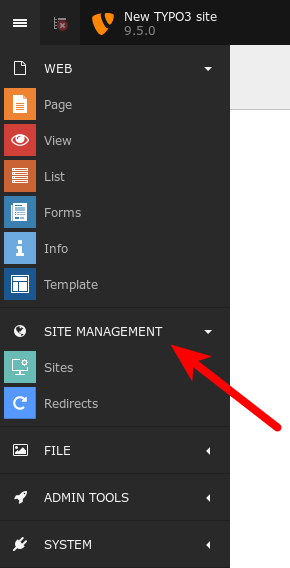
\includegraphics[width=0.45\linewidth]{SiteManagement/83637-AddedNewMainModuleSiteManagement.png}
			\end{figure}
		\end{column}
		\begin{column}{.5\textwidth}
			Die zwei Standardkomponenten sind:
			\begin{itemize}
				\item Sites
				\item Redirects
			\end{itemize}
			\vspace{0.4cm}
			Erweiterungen können bei Bedarf weitere Untermodule hinzufügen.
		\end{column}
		\begin{column}{.1\textwidth}
		\end{column}
	\end{columns}

\end{frame}

% ------------------------------------------------------------------------------
% Site Management -> Sites

\begin{frame}[fragile]
	\frametitle{Site Management}
	\framesubtitle{Site Management → Sites}

	Der Hauptzweck besteht darin, Einstellungen zu speichern, die sich auf die 
	Konfiguration der Site beziehen, z.B. Sprachen, Domains, Routing, Fehlerbehandlung etc.

	\begin{figure}
		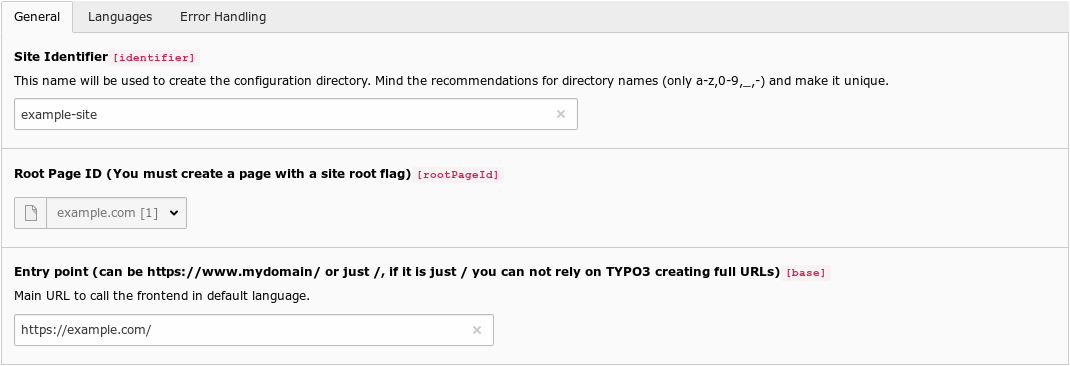
\includegraphics[width=0.8\linewidth]{SiteManagement/SitesModule.png}
	\end{figure}

\end{frame}

% ------------------------------------------------------------------------------
% #83631 - System Extension Redirects Has Been Added

\begin{frame}[fragile]
	\frametitle{Site Management}
	\framesubtitle{Site Management → Redirects}

	Das Modul \textbf{Redirects} ermöglicht Integratoren und Editoren das Konfigurieren 
	von Weiterleitungen. Das Ziel kann eine Seite, eine externe URL, eine Datei usw. sein.

	\begin{figure}
		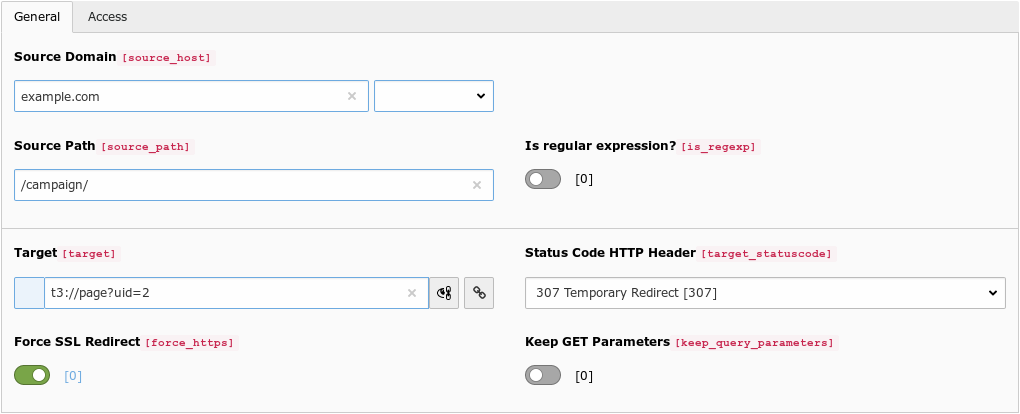
\includegraphics[width=0.8\linewidth]{SiteManagement/RedirectsModule.png}
	\end{figure}

\end{frame}

% ------------------------------------------------------------------------------
% #86422 - TypoScript getText property site

\begin{frame}[fragile]
	\frametitle{Site Management}
	\framesubtitle{Site-Konfiguration in TypoScript}

	% decrease font size for code listing
	\lstset{basicstyle=\smaller\ttfamily}

	Auf die Site-Konfiguration kann über die Eigenschaft \texttt{getText} in TypoScript
	zugegriffen werden:

\begin{lstlisting}
page.10 = TEXT
page.10.data = site:base
page.10.wrap = The base URL is: |

page.20 = TEXT
page.20.data = site:customConfigKey.nested.value
page.20.wrap = The nested value is: |
\end{lstlisting}

\end{frame}

% ------------------------------------------------------------------------------
